
\chapter{知识协同动机因素模型仿真与决策分析}
\label{cha:emulation}

在上一章中,本文提出了个体参与社区知识协同的动机因素模型,描述了动机因
素与协同行为的关系。为了进一步验证模型的有效性,以及利用模型分析社区中
知识协同行为的演化过程,为管理决策提供依据,需要对模型进行仿真实验。

\section{动机因素模型仿真}

\subsection{仿真的基本过程}
建立模型要素的因果回路是模型仿真的第一步。但是仅靠因果回路图是无法进行
仿真的。因果回路图的适用范围是表达系统要素间的关联和反馈过程,但是变量
的性质却未能因果回路图中并没有表现出来。因果回路图无法描述系统管理和控
制过程,因此被应用于早期建模过程中,重点反应最基本的模型结构,方便建模
者对模型主体的把握。

流量和存量是社会经济系统中的两种基本变量。存量反映了系统在某一时刻的状
态,而流量则揭示了存量的变化快慢情况,这在因果图中是无法体现出来的。存
量变化的速率是系统演化的重要决定因素之一。因此,区分存量和流量是对因果
关系更细致和深入的描述,反应系统中各要素的控制与反馈。在存量流量模型的
基础上,通过设定各个变量的初值,步长等参数,用方程来描述各因素间的函数关
系,最终得到系统仿真的模型。通过多次试运行和调整,以及对模型进行有效性
检验,使模型可以较准确地反映现实世
界的变动,研究者可以利用模型进行决策分析。模型仿真的基本过程如图\ref{fig:vensim}所示。
\begin{figure}[htb]
  \centering
  \scalebox{0.7}{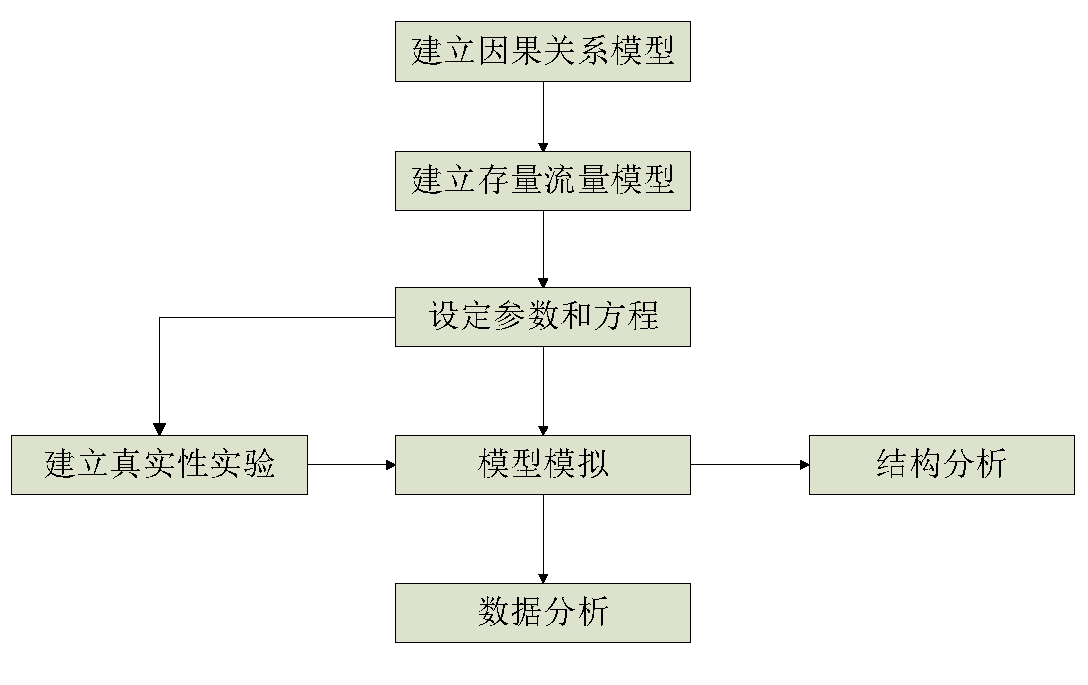
\includegraphics{vensim.pdf}}
  \caption{\small{\textbf{模型仿真过程}}}
  \label{fig:vensim}
\end{figure}
\subsection{动机因素存量流量图}

在因果图中,不论是动机因素,还是个体的行为都是系统的状态,是存量。为了
描述动机于行为间的关系而故意忽略了一些流量变量和外生变量。但是,这些被
忽略的变量对于整个系统起到了重要作用,没有这些变量系统就不可能正确地表
示现实系统的运行。

对于大部分动机因素,它们和个体的行为之间构成了一个正反馈回路和一个负反
馈回路,既动机的
增强会提升个体的行为水平,如果协同行为的得到了他人的正反馈,则会提升个体的动
机;反之如果协同行为得到了他人的负反馈,个体的动机会受到伤害。对于现实
系统来说,有几个重要的变量未能包含在因果图中。首先,个体的协同行为水平
不仅受到动机的影响,还受到其他因素,尤其是个体工作能力的限制。无论个体怎么
提升协同水平,都不可能超过个体的最大工作能力。这就是所谓“增长的极限”。
个体的最大工作能力是行为水平的抑制因素,使得行为水平不可能无限制地增长
下去。其次,动机作为系统中的存量,必然要受到流量的影响。动机的流
入是从协同活动中获得的正反馈转化的动机,动机的流出则是协同活动中获得的
负反馈使动机削弱的数量。流入水平和流出水平综合决定了动机存量的变化。第
三,不论是动机转化为行为还是行为的结果反馈影响动机都不是线性过程。这种
变换也存在遍及递减效应,动机的水平越高,每增加一单位动机所能引起的行为
水平的增加就越少。因此如果仅考虑行为与动机的互动关系的话,个体的动机应
该呈对数增长(或减弱),最后接近某个极大(小)值。最后,成就动机同其他
动机略有不同。成就动机促使个体参与某种活动从中获得成就感。成就感的提升
削弱成就需求。但是成就感有一种随时间自动削弱的属性,在没有任何外力介入
的情况下成就感将逐渐流失,从而提升了个体的成就需求,促使他们参与新的活
动重新获得成就感。流失速度的不同决定了不同人的行为模式,对于流失速度快
的人来说,他们从参与活动中所获得的成就感迅速减少,因此这些人表现为进取
精神非常强,不停地追逐新的目标来满足自己对成功的渴望。而流失速度慢的人则
会很长时间满足于自身取得的成就,表现为为止步不前,不愿接受新的挑战。

根据以上分析的结果,本文将把因果关系图转换为存量流量图,同时在模型中加
入新的变量,使模型更符合现实世界。因为转换的模型力图完整描述存量于流量
的关系,因此对因果关系进行了简化处理。变量间具体、详细的因果关系请参考
因果关系图。大部分的动机因素都有同样的特征:动机增加引起行为水平的提升;
如果行为得到正反馈则会促使动机也得到相应的提升,负反馈则会使动机减弱。。对于利他主义和感知到的意义两类动机由
于和行为之间是单向关系,行为的结果不会对这两个变量产生。影响。成就动机和认知失调两类动机有
各自的特点:成就动机根据满足感的变化而变化;认知失调的变化方向则和其他
因素相反,正反馈会减少认知失调水平,从而降低个体动机。在模型中引入了流量变量“每次协同行为增加的动机”表示
动机的流入,“他人对个体的协同行为减少的动机”表示动机的流出,以此表示
动机的动态性;引入变量“疲劳“和外生变量“个人工作的最大能力”构建行为
的负反馈闭环,反应行为水平受到抑制的特征。引入流量变量“满足感的流失”
反应满足感随时间减少的特点。转换的存量流量图如图
\ref{fig:refined-model}和图\ref{fig:refined-model2}所示。
\begin{figure}[!htb]
  \centering
  \scalebox{0.59}{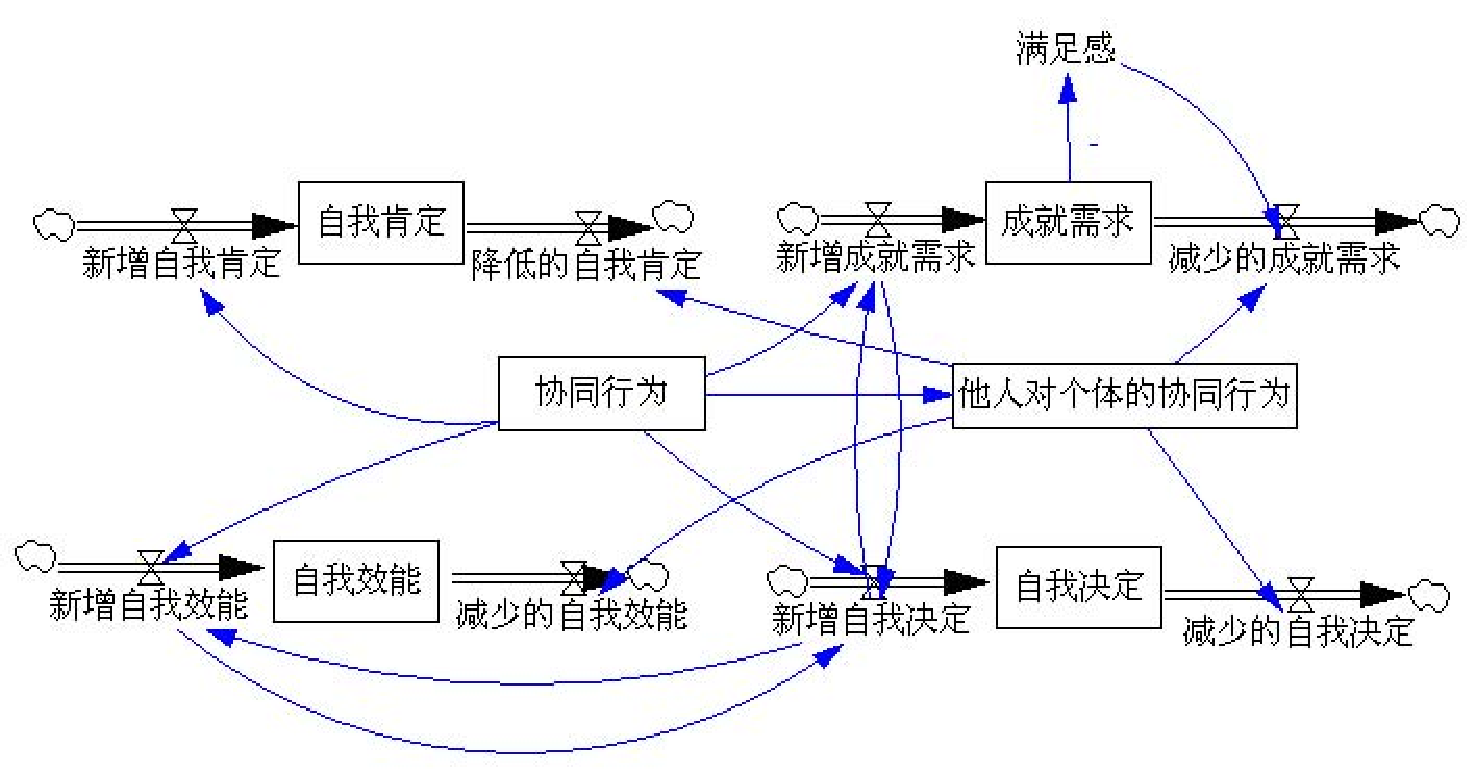
\includegraphics{io1.pdf}}
  \caption{\small{\textbf{知识协同个体动机因素的存量流量图}}}
  \label{fig:refined-model}
\end{figure}

\ref{fig:refined-model}所示。
\begin{figure}[!htb]
  \centering
  \scalebox{0.59}{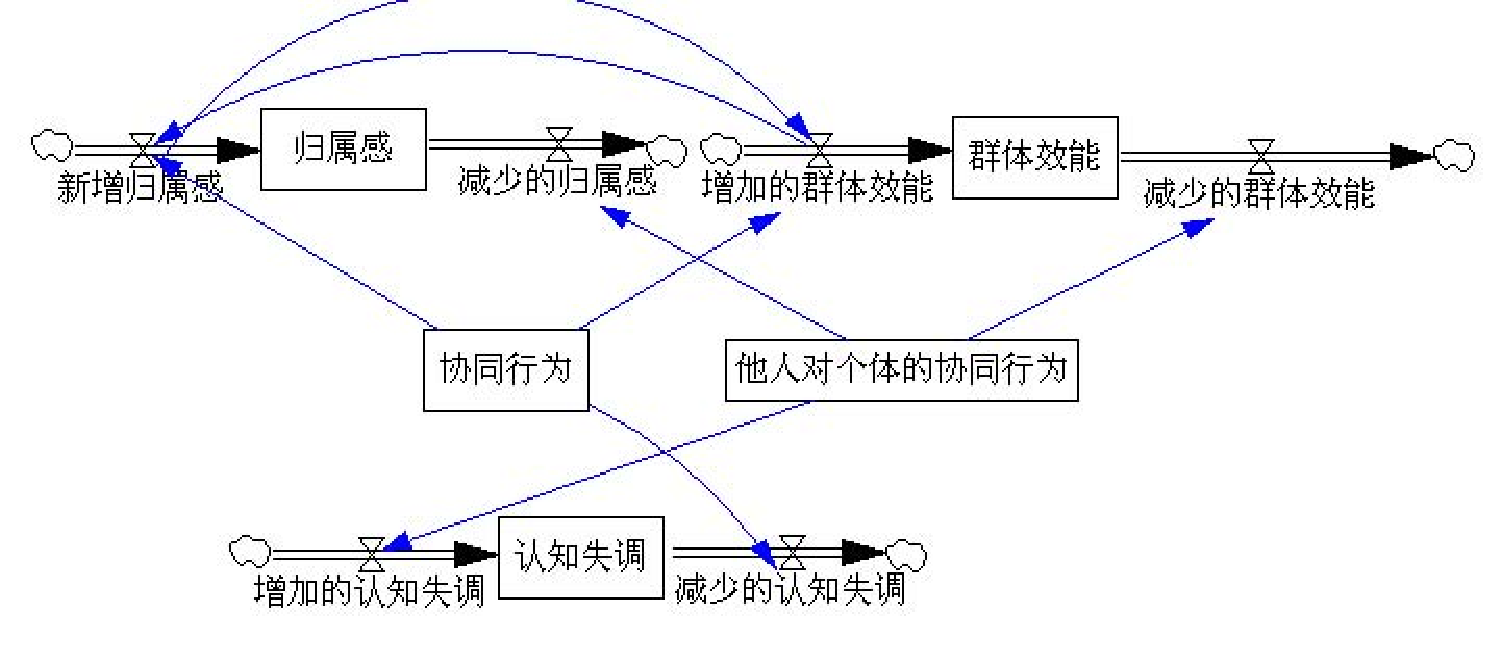
\includegraphics{io2.pdf}}
  \caption{\small{\textbf{知识协同人际间动机因素的存量流量图}}}
  \label{fig:refined-model2}
\end{figure}

\subsection{模型方程的设置}

每个变量都和其他变量形成一定的函数关系,这种关系使用方程来表示。下面列
举了了模型中所有涉及到的方程。其中称领导者和领域专家的模型为模型1,内
容贡献者、维护者和边缘用户的模型为模型2.
\begin{enumerate}
\item 模型1行为水平=转换水平$_1$$\times (\sum$成就动机+利他主
  义+感知到的意义+自我决定+自我效能+自我肯定)
\item 模型2行为水平=转换水平$_1$$\times (\sum$成就动机+利他主
  义+感知到的意义+自我决定+自我效能+自我肯定+认知失调+群体效能+归属感)
  
\item 成就需求=个体的最大成就需求-满足感$\times$转换系数+本期自我决定
  增量$\times$转换系数
\item 自我决定=上一期自我决定+正协同贡献$\times$转换系数+负协同贡献
  $\times$转换系数+本期自我效能增量 $\times$转换系数+本期归属感增量$\times$转换系数
\item  自我效能=上一期自我效能+正协同贡献$\times$转换系数+负协同贡献
  $\times$转换系数+本期自我决定增量 $\times$转换系数
\item 自我肯定=上一期自我肯定+正协同贡献$\times$转换系数+负协同贡献
  $\times$转换系数
\item 认知失调=他人的协同行为$\times$转换系数+他人对个体的协同行为
  $\times$转换系数-协同行为水平$\times$转换系数
\item 群体效能=上一期群体效能定+正协同贡献$\times$转换系数+负协同贡献
  $\times$转换系数+本期归属感增量$\times$转换系数
\item 归属感=上一期归属感+正协同贡献$\times$转换系数+负协同贡献
  $\times$转换系数+本期自我效能增量 $\times$转换系数+本期群体效能增量 $\times$转换系数



\end{enumerate}

\subsection{参数估计}
参数估计是建立系统动力学模型重要的过程。即使是参数值的微小变化,也可能会引起系统
行为产生较大幅度的波动,甚至改变整个系统行为的极
性。因此, 为保证模型模拟结果与真实系统的一致性, 应尽可能地准确估计模型
的参数。

模型的参数估计是模型的局部分别独立地进行,然后在总体模型进行模拟仿真时
在进行总的调试。系统动力学本身并不限制参数估计的方法,可以根据需要和具
体情况灵活地选用不同的参数估计方法。参数估计的完成标志着模型从定性向定
量的转化。

参数的估计方法可以分为以下几种。
目前SD 模型参数估计的技术大致可分为3 种[1, 2 ]: (1) 单个参数、表函数关系、间接计算等基于利用
模型变量集结程度以下的数据进行的估计; (2) 运用单方程进行估计; (3) 运用多方程进行估计等. 其中后
2 种都是基于与模型变量集结程度相当的数据进行的估计. 此外, 还可以运用统计技术进行估计.
但是, SD 模型基于结构而不是统计相关性的特征, 使得它所要求的许多参数(如国民经济系统中描述
人均国民收入对积累率影响程度的参数等) 往往缺乏可资利用的资料, 使建模工作者可以有效地运用前述
的种种方法对它们进行合理的估计. 还有一种情况, 由于SD 模型所处理的常是具有多重反馈的复杂系
统, 这使得处在因果链上相隔甚远的变量间的关系变得很不直观甚至反直观, 要估计描述它们对应关系的
参数也十分困难. 为了对这些难以估计的参数进行估计, 有时就得采用“仿真—分析—修正”这种类似于手
工式的“试凑法'' \cite{linwenhao2002}。

参数的估计工作分为两部分,一部分是估计变量的初值,另一部分是估计方程中
的参数。在动机因素于协同行为的模型中,大部分变量都是定性变量,本身就难
于量化。在缺乏资料的情况下,将定性变量数量化,本身就带有一定的盲目性和
随意性,因此手工调试是必不可少的环节。但是,通过使用一定的估计方法能大
大简化手工调试的工作量,减少调试的时间。

参数估计的结果如表\ref{tab:initail-value-level}和表\ref{tab:initail-value-transe}所示。
\begin{table}[!htbp]
  \centering
\small
  \caption{\small{\textbf{状态变量参数初始值}}}
% Table generated by Excel2LaTeX from sheet 'Sheet2'
\begin{tabular}{|c|c|c|c|c|c|}
\hline
\multicolumn{ 1}{|c|}{变量名称} &                                     \multicolumn{ 5}{|c|}{初始值} \\
\hline
\multicolumn{ 1}{|c|}{} &        领导者 &       领域专家 &      内容贡献者 &      内容维护者 &       边缘用户 \\
\hline
      利他主义 &      13      &        13    &        10    &   10         &      10      \\
\hline
    感知到的意义 &      10      &     10       &     10       &   10         &      10      \\
\hline
      自我决定 &      20      &     18       &      15      &          10  &    10        \\
\hline
      自我效能 &     25       &      15      &        15    &        8    &       5     \\
\hline
      自我肯定 &      25      &    15        &     10       &      10      &       10     \\
\hline
      成就需求 &     20       &     18       &      18      &      5      &        5    \\
\hline
      认知失调 &     $\slash$       &       $\slash$       &      10      &       15     &      9      \\
\hline
      群体效能 &     $\slash$         &          $\slash$    &    15        &      10      &       5     \\
\hline
       归属感 &       $\slash$       &     $\slash$         &      18      &        18    &        5    \\\hline
\end{tabular}  


  \label{tab:initail-value-level}
\end{table}

\begin{table}[!htb]
  \centering
\caption{\small{\textbf{转换系数初始值}}}
\small
% Table generated by Excel2LaTeX from sheet 'Sheet2'
\begin{tabular}{|c|c|c|c|c|c|}
\hline
\multicolumn{ 1}{|c|}{变量名称} &                                     \multicolumn{ 5}{|c|}{初始值} \\
\hline
\multicolumn{ 1}{|c|}{} &        领导者 &       领域专家 &      内容贡献者 &      内容维护者 &       边缘用户 \\
\hline
自我决定到协同水平的转换系数 &     0.003       &     0.003       &      0.002      &      0.001      &     0.001       \\
\hline
自我效能到协同水平的转换系数 &      0.005      &    0.005        &      0.006      &      0.008      &        0.008    \\
\hline
自我肯定到协同水平的转换系数 &      0.002     &       0.002    &      0.001      &     0.001       &       0.001     \\
\hline
成就需求到协同水平的转换系数 &     0.008       &     0.008       &     0.004       &         0.002   &       0.001     \\
\hline
认知失调到协同水平的转换系数 &      $\slash$       &    $\slash$         &    0.002        &         0.003   &      0.004      \\
\hline
群体效能到协同水平的转换系数 &          $\slash$    &       $\slash$       &   0.003         &    0.003        &        0.002    \\
\hline
归属感到协同水平的转换系数 &        $\slash$      &      $\slash$        &      0.003      &     0.003       &   0.003         \\
\hline
正协同贡献到自我决定的转换系数 &    0.0015        &    0.0014        &      0.0009      &        0.0006    &      0.0006      \\
\hline
正协同贡献到自我效能的转换系数 &    0.0022        &      0.0018      &       0.0013     &       0.0009     &  0.0009          \\
\hline
正协同贡献到自我肯定的转换系数 &     0.0014       &        0.0013    &     0.001       &        0.0006    &     0.0006       \\
\hline
正协同贡献到成就需求的转换系数 &       0.0008     &        0.0008    &      0.001      &       0.0008     &       0.0008     \\
\hline
正协同贡献到认知失调的转换系数 &     $\slash$        &     $\slash$        &    0.0007        &     0.0005       &       0.0006     \\
\hline
正协同贡献到群体效能的转换系数 &   $\slash$          &   $\slash$          &      0.0005      &     0.0005       &      0.0003      \\
\hline
正协同贡献到归属感的转换系数 &    $\slash$         &      $\slash$       &       0.0004     &      0.0005      &      0.0002      \\
\hline
负协同贡献到自我决定的转换系数 &     0.0001       &     0.0001       &    0.0005        &      0.0008      &     0.0009       \\
\hline
负协同贡献到自我效能的转换系数 &      0.0001      &     0.0001       &    0.0004        &      0.0009      &        0.001    \\
\hline
负协同贡献到自我肯定的转换系数 &     0.0001       &      0.0001
&0.0005&  0.0006            &  0.0006          \\
\hline
负协同贡献到成就需求的转换系数 &      0.0002      &       0.0002     &     0.0003       &       0.0003     &      0.0003      \\
\hline
负协同贡献到认知失调的转换系数 &       $\slash$      &    $\slash$         &    0.0002        &     0.0002       &     0.0001       \\
\hline
负协同贡献到群体效能的转换系数 &   $\slash$          &       $\slash$      &    0.0002        &       0.0002     &    0.0002        \\
\hline
负协同贡献到归属感的转换系数 &      $\slash$       &       $\slash$      &      0.0001      &        0.0003    &      0.0003      \\
\hline
\end{tabular}  

  
  \label{tab:initail-value-transe}
\end{table}

\section{模型检验}

当模型的所有参数都确定后,需要测试模型的有效性,检查模型是否能较准确地
模拟现实系统。模型的检验是一个不断证伪的过程。常见的检验方法包括结构评
价测试、参数估计测试、行为重现测试、灵敏度测试、系统改进测试等。检验往
往是通过同用户、专家的不断对话,深入理解系统行为,同时检查系统的因果关
系是否合理,方程量纲是否一致,对模型进行各种条件下的测试,并对比模型的
运行结果和实际数据。本文在参考大量文献的基础上,借鉴了其他学者的实证研
究成果,对模型进行直观检验,观测模型是否能重现真实系统中的行为变化。

模型是现实世界的简化和抽象,因此一个模型不可能精确地再现现实中的各种现
象。模型的主要目的在于反映趋势的变化。为了验证模型的正确性,本文将模型
仿真数据同真实数据进行对比。针对不同类型的用户,使用维基百科提供的数据分别计算了连续40个月的
月人均贡献度和仿真结果进行比对。

图\ref{fig:simu1}是领导者用户的仿真结果和真实数据图。从图中可以看出,领导者用户的月人
均贡献度呈现出比较明显的对数函数特征,而仿真的结果显示为系统行为呈现出
寻的模式,因此虽然模型同实际数据有误差,但是仍然较准确地再现了现实趋
势,可以使用模型模拟用户的知识协同行为。

\begin{figure}[!htb]
  \centering
  \scalebox{0.65}{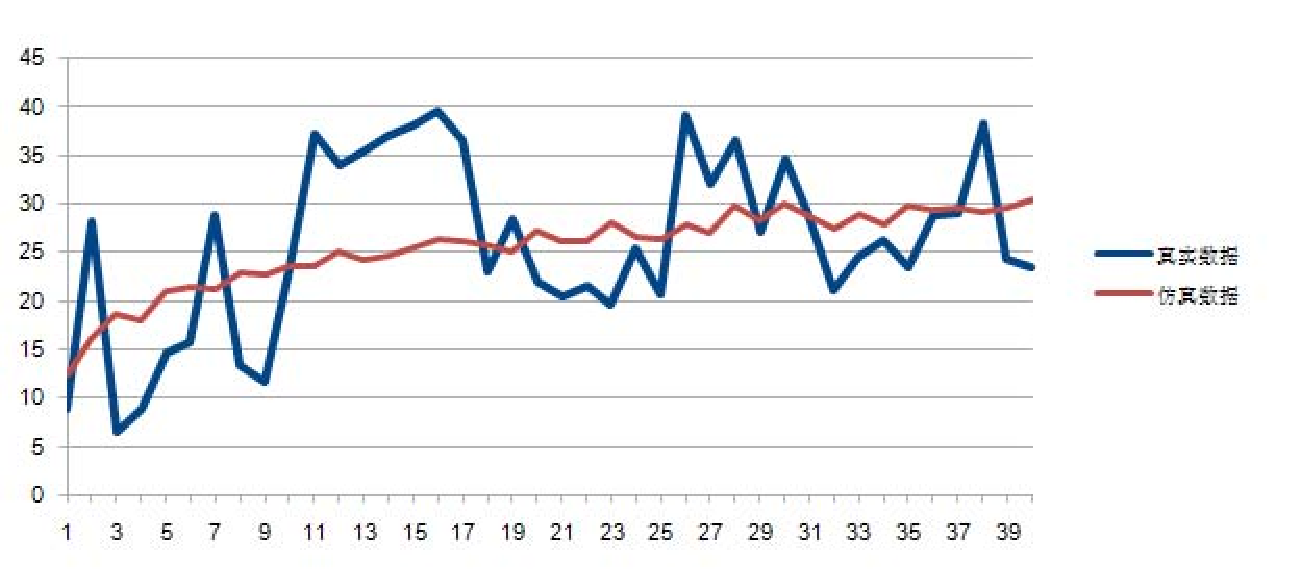
\includegraphics{simu-1.pdf}}
  \caption{\small{\textbf{领导者用户仿真结果}}}
  \label{fig:simu1}
\end{figure}

图\ref{fig:simu2}是领域专家用户的仿真结果和真实数据图。真实数据反映出该类用户的月人均
贡献度在初期显著下降后迅速进入一个平稳状态。仿真结果则表现为一个递减
的对数函数。两者的趋势是一致的。

\begin{figure}[!htb]
  \centering
  \scalebox{0.65}{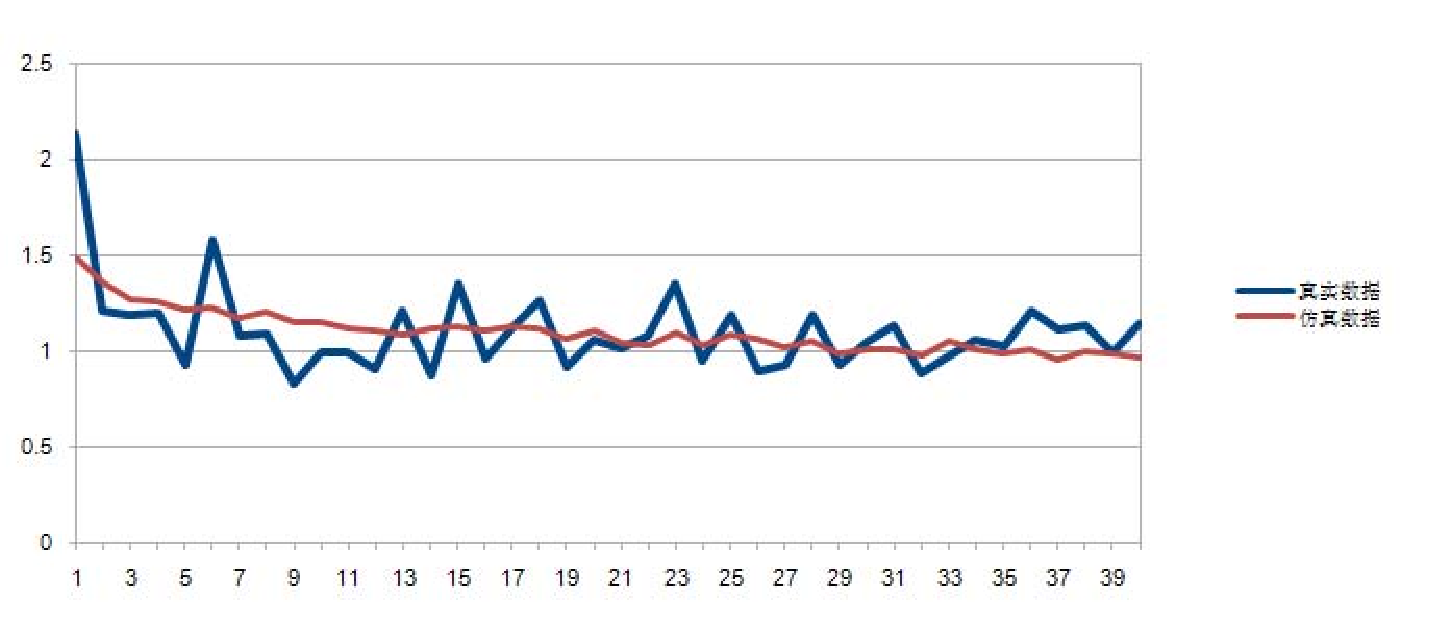
\includegraphics{simu-2.pdf}}
  \caption{\small{\textbf{领域专家用户仿真结果}}}
  \label{fig:simu2}
\end{figure}

图\ref{fig:simu3}是内容贡献者的仿真结果和真实数据图。内容贡献者的月人均
贡献度非常平稳,没有明显的震荡。仿真的结果也几乎是一条直线,同实际数据
的拟合度很高。因此模型很好地反映了内容贡献者的动机与知识协同水平的相互
作用。

\begin{figure}[!htb]
  \centering
  \scalebox{0.65}{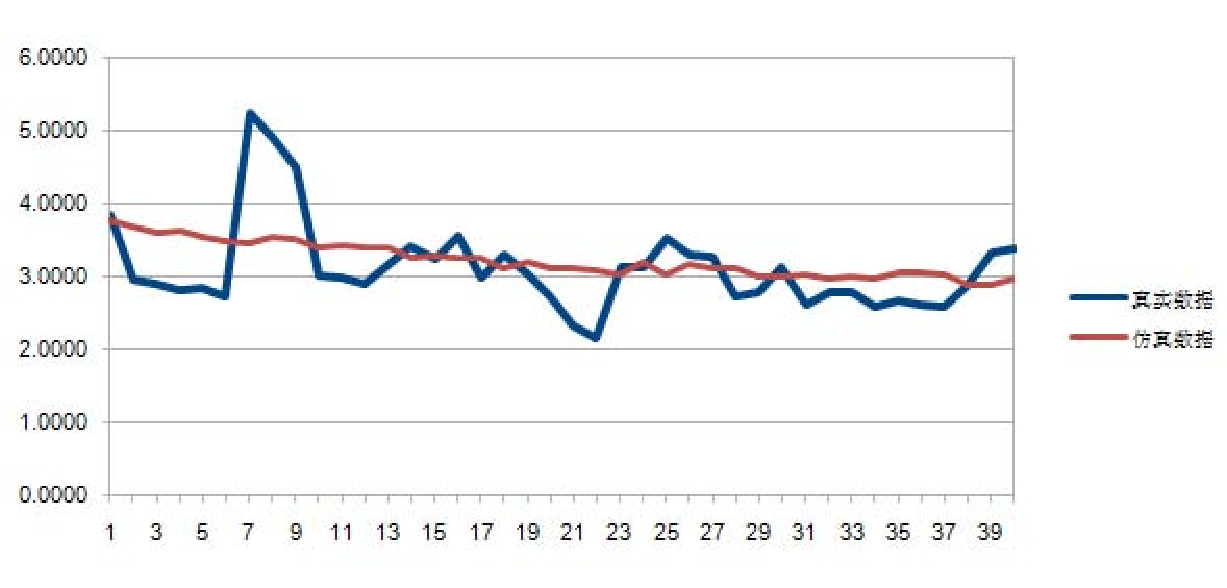
\includegraphics{simu-3.pdf}}
  \caption{\small{\textbf{内容贡献者用户仿真结果}}}
  \label{fig:simu3}
\end{figure}

图\ref{fig:simu4}是内容维护者的仿真结果和真实数据图。实际数据显示内容
维护者的月人均贡献很快下滑,随后逐渐平稳,下滑趋势减缓。仿真数据则是一
条对数曲线,除了和个别真实点的数据结果差距很大以外,整体的拟合度很高,
说明模型对于分析内容维护者的行为是有效的。
\begin{figure}[!htb]
  \centering
  \scalebox{0.65}{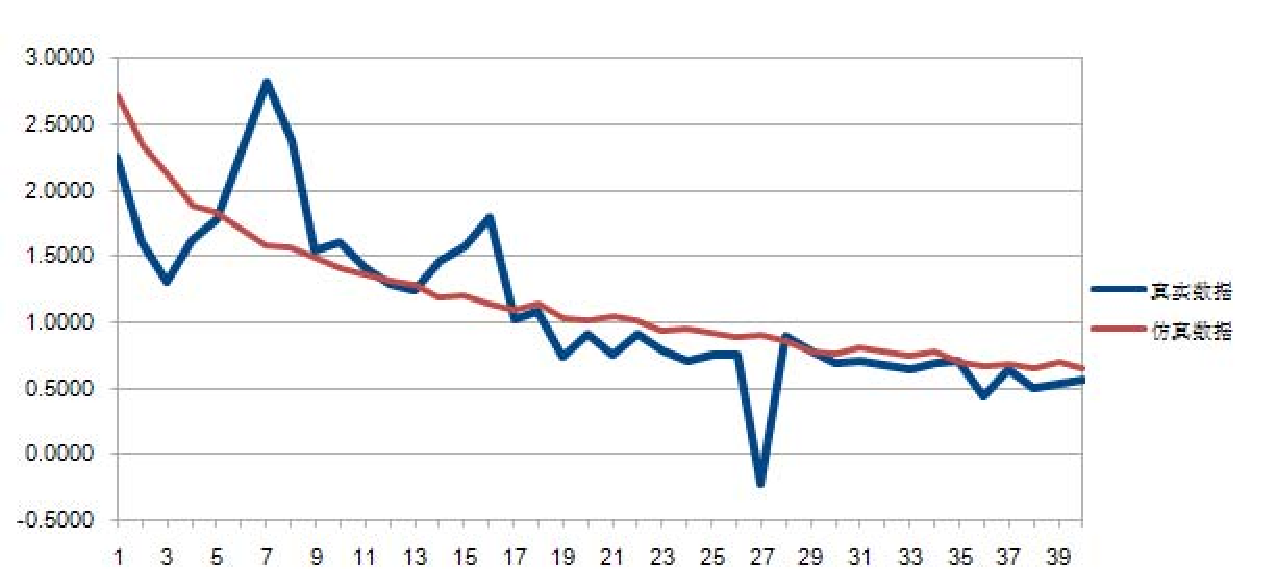
\includegraphics{simu-4.pdf}}
  \caption{\small{\textbf{内容维护者用户仿真结果}}}
  \label{fig:simu4}
\end{figure}

图\ref{fig:simu5}是边缘用户的仿真结果和真实数据图。边缘用户的月人均贡
献值是所有用户类型中最为特殊的:呈加速下滑趋势。模型仿真结果也显示月人均贡献是一条近
似于指数函数的曲线。虽然真实数据的波动水平比较大,但是模型的拟合结果仍
然反映了真实系统的变动趋势。
\begin{figure}[!htb]
  \centering
  \scalebox{0.65}{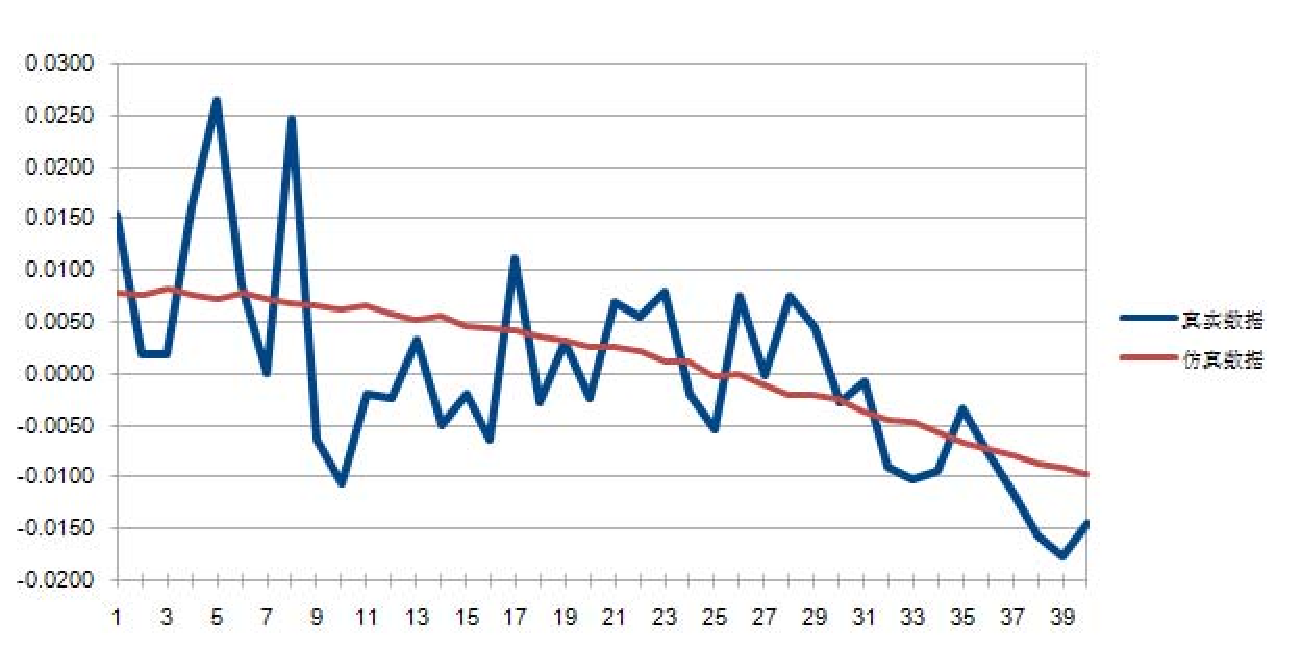
\includegraphics{simu-5.pdf}}
  \caption{\small{\textbf{边缘用户仿真结果}}}
  \label{fig:simu5}
\end{figure}

\section{动机因素模型分析}
通过对比模型仿真结果和实际数据,可以判定模型基本反映了维基百科社区中各
类用户的知识协同动机和行为间的关系。利用仿真模型可以进一步分析用户的协
同模式、预测协同行为以及提出相应的管理建议。

\subsection{领导者用户}

领导者用户是整个用户群体中最积极、投入程度最高的群体。个体的人均贡
献远远要高于其他类型的用户。从图中可以看到,尽管有比较明显的波动,但是
月人均贡献还是接近30。领导者用户能有如此高的行为水平和其很强的参与动机是分
不开的。同时,领导者用户的水平很高,其参与的内容绝大部分都受到了其他用
户的认同。因此,协同行为于协同动机形成了正反馈环,使得领导者用户的月人
居贡献不断提高。但是,依据系统动力学原理,正反馈环所造成的良性循环应该
程指数增长,意味着月人均贡献应该是加速上扬的。但是数据显示,领导者用户
的月人均贡献虽然也在上升,但是上升速度确实不断递减的,到最后几乎停滞下
来。

造成这种情况的原因可能有两个:一种是系统本身的主导反馈是负反馈。同正反
馈不同,负反馈回路追求系统的平衡和停滞,一旦系统发生状态偏离,负反馈回
路将使其回到预定的目标或状态。另一种可能是系统的增长模式为S型增长。S型
增长产生的原因是系统中同时存在多个正反馈回路和负反馈回路。当增长达到一
定程度时,负反馈回路开始发挥作用一致增长,是增长不会一直持续下去。最
后,一个或多个条件约束将使增长停止。

根据领导者用户的行为特征,影响领导者的协同贡献的不太呈现完全的负反馈形
式。由于数据选取的时间段为领导者用户已经参与社区的中后期,考虑到较高的
协同贡献,说明领导者用户的月人均协同贡献应该是S型增长,并且到了增长的
末期。在领导者用户的因果回路图中,个人的最大工作时间回路是一个负反馈回
路。当用户的投入水平不断增强,该回路的作用也越来越明显。不管用户
的动机水平有多高,协同行为水平也不可能突破最大工作时间的限制,这时用户
已经是“心有余而力不足”,最终导致了协同贡
献增长的停滞。

为了验证这一点,本文做了两个仿真实验。首先将所有的用户动机程度提升
$10\%$,如果个体的协同行为已经达到了最大值,那么即使提升个体的协同动机
也不可能使协同贡献得到提升。仿真结果如图\ref{fig:improve1}所示。

\begin{figure}
  \centering
  \scalebox{0.65}{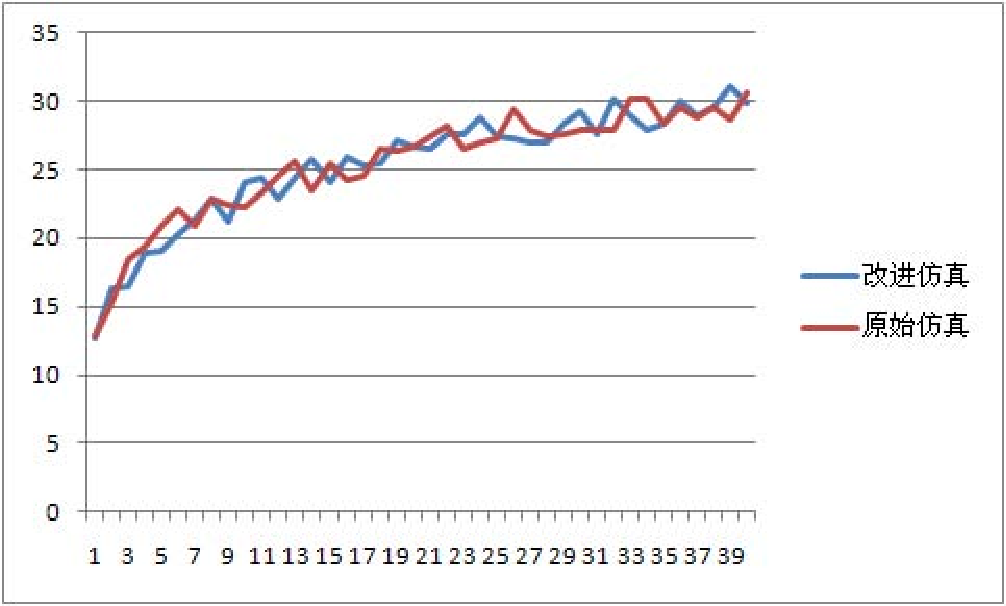
\includegraphics{improve1.pdf}}
  \caption{\small{\textbf{提升领导者用户初始动机的仿真结果}}}
  \label{fig:improve1}
\end{figure}

从图中可以看出,领导者用户的月人均协同贡献几乎没有变化,这意味着协同动
机的提升对行为已经不能产生影响。接下来,保持其他条件不变,将个体的最大
工作时间加大$10\%$,尽管这已经同现实情况不相符,但是可以借由模拟观察到
最大工作时间对协同行为的限制。仿真结果如图\ref{fig:improve2}所示。

\begin{figure}
  \centering
  \scalebox{0.65}{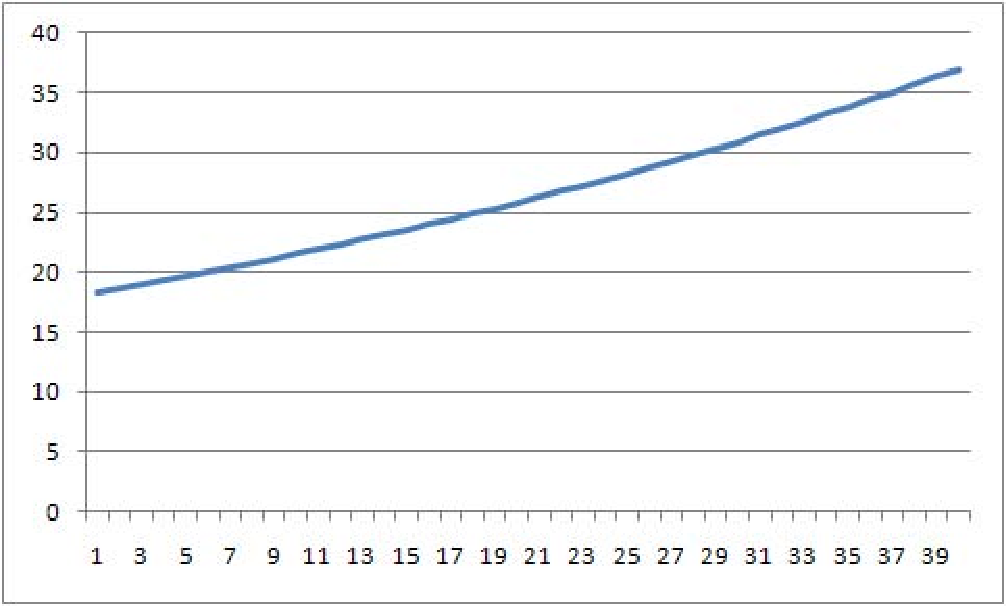
\includegraphics{improve2.pdf}}
  \caption{\small{\textbf{提升领导者用户最大工作时间的仿真结果}}}
  \label{fig:improve2}
\end{figure}

在提升了个体的最大工作时间后,个体的贡献显著增长,同时增长的速度呈增加
的趋势。这证明了个体的协同行为确实受到了该因素的制约,使得贡献形成了S
型增长。随着时间推移,个体的贡献将稳定维持在一个较高的水平,除非外界因
素发
生明显的变化,否则不会发生太大的波动。

领导者用户主要受到个体层次的动机驱动参与知识协同,他们在很短的时间内就
达到了个人能力的最大值。为了维持领导者用户的参与水平,社区所能采取的措施和其他群体
有显著的不同。激励措施对于领导者用户并不重要,即使动机水平再高也不能提
升其参与程度。社区所要做的应该是保护用户的热情,不要使社区中的一些负面
因素降低参与者的动机。领导者用户是真正希望从工作中获得快乐的一类用户,
如果他们不能从中获得满足感,则参与动机会很快消失。为此,社区应该多听取
用户意见,把握好社区发展的方向,尽力满足用户需求,努力维护用户的动机不
受到伤害。同时社区应该注意到,尽管领导者用户是社区的核心力量,但是其他
类型用户的作用也不应该被忽视。如果社区不能平衡核心用户的需求和其他成员
的利益,那么社区的发展会受到很大的制约。

\subsection{领域专家用户}
领域专家用户同领导者用户有着相似的协同模式,同时他们对于所参与的条目也
有极高的贡献度。但是,领域专家用户的月人均贡献却和领导者用户大相径庭,
不但数值很低,而且呈递减趋势,最后到1左右稳定下来。贡献度的下降趋势显
示了对数函数的特征,模型仿真的结果说明用户协同贡献的变化符合寻的模式,即负反馈成
为了领域专家动机和行为间关系的主导关系。

在因果模型中存在两个负反馈环:一个是个体最大工作时间的负反馈环,另一个
是成就动机的负反馈环。前者限制了协同行为的最大水平,后者则有可能改变整
个因果链的主导关系。考虑到领域专家用户的月人均贡献非常低,因此决定行为
模式的负反馈环是最大工作时间的可能性不大,也就是说用户的实际能力还远远
没有发挥出来。真正影响用户协同水平的是成就动机。成就需求在个体完成任务
的过程中得到满足,这种满足感会削弱成就动机,从而降低个体的协同参与水平。
成就动机成为主导的负反馈环有两个必要条件:首先成就动机的初始值必须很
高,这样成就动机的重要性才能超过其他动机;其次满足感必须持续处于较高水
平,也就是成就感的流失非常慢。只有这样,个体的动机才会以成就动机为主,
同时成就需求可以在较长时间段内得到满足,降低了个体的协同行为水平。 

以上推断可以利用仿真来验证。图\ref{fig:improve4}是将领域专家用户所有的
动机因素水平提升$20\%$后得到的结果。结果显示用户的协同水平有所提高,说
明提升动机因素水平是有作用的。但是,协同水平的变化趋势仍然没有改变,还
是呈现缓慢下降的趋势。这意味着负反馈的力量依然强大。消除负反馈的影响而
不是激励用户提升其动机水平是改进领域专家用户绩效行之有效的方法。
\begin{figure}[!htb]
  \centering
  \scalebox{0.65}{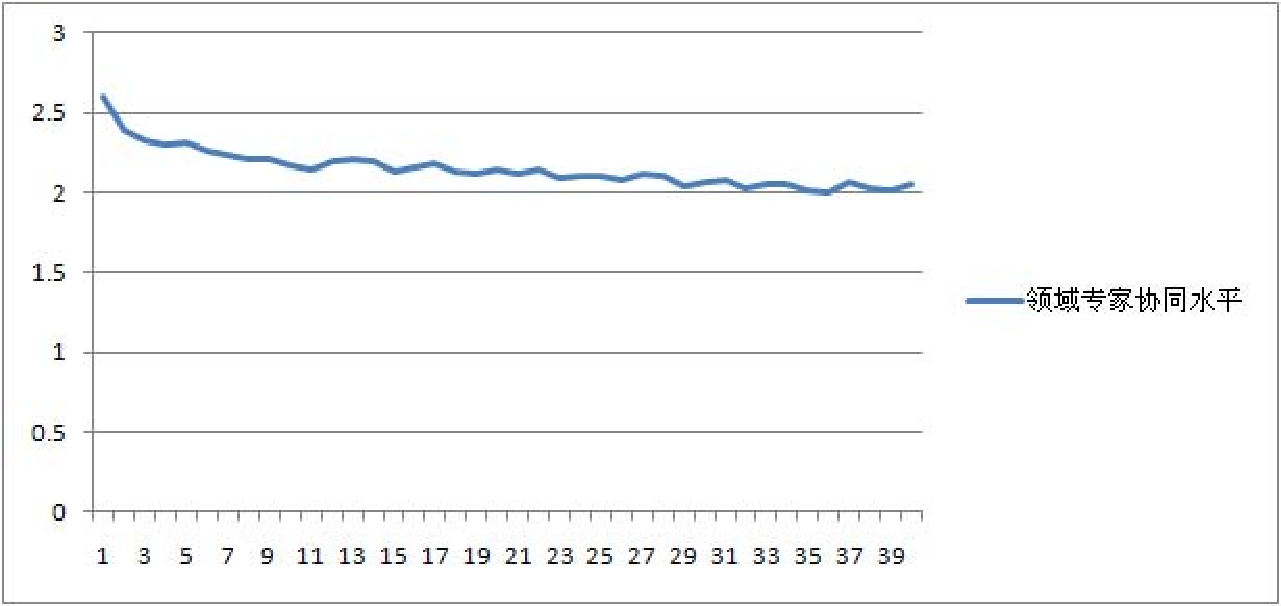
\includegraphics{improve4.pdf}}
  \caption{\small{\textbf{提升领域专家所有动机的仿真结果}}}
  \label{fig:improve4}
\end{figure}

%图是领域专家用户和领导者成就感变量的仿真结果。可以看到领域专家的成就
%感一直处在非常高的位置,而领导者的成就感则稳定在一个很低的水平。
图\ref{fig:improve3}是将领域专家用户除了成就需求以外的其他动机因素提升$10\%$
的结果。提升后贡献值的趋势发生了较大的变化,不在是逐步下降,而是稳步上
升。这两个仿真结果揭示了两类用户的根本差异。领域专家用户的成就需求在所
有动机中占了较大的比重,也就说领域专家用户相对来说更注重成就的取得。但
是,该类用户的成就感消失的很慢,他们在协同过程中迅速满足了自身的成就需
求,并且一直在享受所取得的成就。相比之下,领导者用户的成就感很快消失,
能使其一直保持参与知识协同的动力。

\begin{figure}[!htb]
  \centering
  \scalebox{0.65}{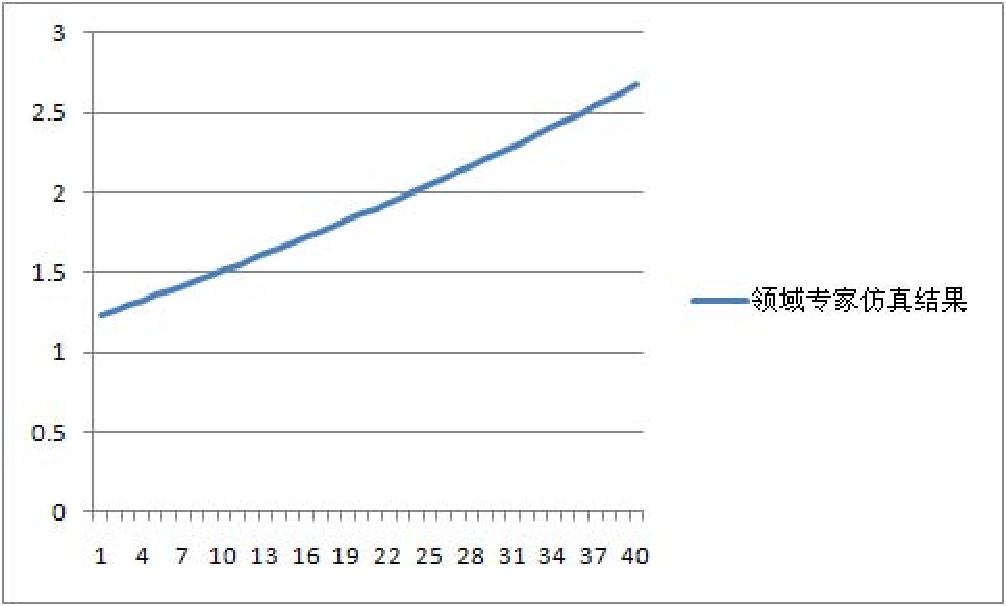
\includegraphics{improve3.pdf}}
  \caption{\small{\textbf{提升领域专家成就动机的仿真结果}}}
  \label{fig:improve3}
\end{figure}

领域专家用户具有和领导者相似的协同模式和个人能力,但是其容易“自满”的
特点限制了其发挥自身的最大能力。如果社区能够采取措施将领域专家转化为领
导者,那么对于社区的发展将是大有裨益的。首先,应该加强领域专家用户的成
就期待感,让他们认识到仅仅完成一两个条目的撰写还远远不是成功的终点,只
有唤起他们更大的成功欲望,才能有效地克服“自满”情绪。同时,社区给与这
类用户充分的支持和鼓励,这样有助于调整内部动机各个因素间的比率,降低成
就需求的比重,使那些具有正反馈关系的动机占据主要地位,最大限度地提升领
域专家用户的参与水平。

\subsection{内容贡献者}

内容贡献者是社区的中坚力量。个体层面的动机和群体层面的动机都会影响他们
参与知识协同的程度。内容贡献者的月人均贡献度的变化很平缓,但是仍然可以
看到加速上升的趋势,这意味着正反馈对协同水平起到了主要作用。同时,内容
贡献者的贡献度水平非常高,在所有用户群体中仅次于领导者用户。因此,这类
用户并不存在领域专家那种容易“自满”的特点。

尽管内容贡献者的贡献度呈现指数增长的特点,但是其增长速度非常缓慢。通过
对比其月度的总贡献和月度的正贡献可以发现:总贡献和正贡献的值非常接近,
就平均水平而言,正贡献与总贡献的差小于$10\%$,而二者最大的差值仅为
$18\%$。这意味着内容贡献者的工作水平非常高,大部分编辑内容都被其他协同
着接受而得以保留。因此内容贡献者所得到的负反馈实际上是非常少的。造成内
容贡献者贡献增长较慢的主要原因是其动机的初始值较低。只有在经历较长时间
后,正反馈的效应才能逐渐体现出来。内容贡献者同领导者用户不同,他们的动
机水平是在协同过程中不断获得正反馈得到的,而不是一开始就有很强的动机。
以下两个仿真验证了这一点。

图\ref{fig:improve5}是将所有的个体层次动机的初始值提升了$10\%$后的仿真结果。动机提升后个
体的贡献度有了一定的提高,同时随时间加速上升的趋势也要比提升前明显。这
个结果证明如果初始动机水平高,那么参与水平的提升速度也会提高。

\begin{figure}[!htb]
  \centering
  \scalebox{0.65}{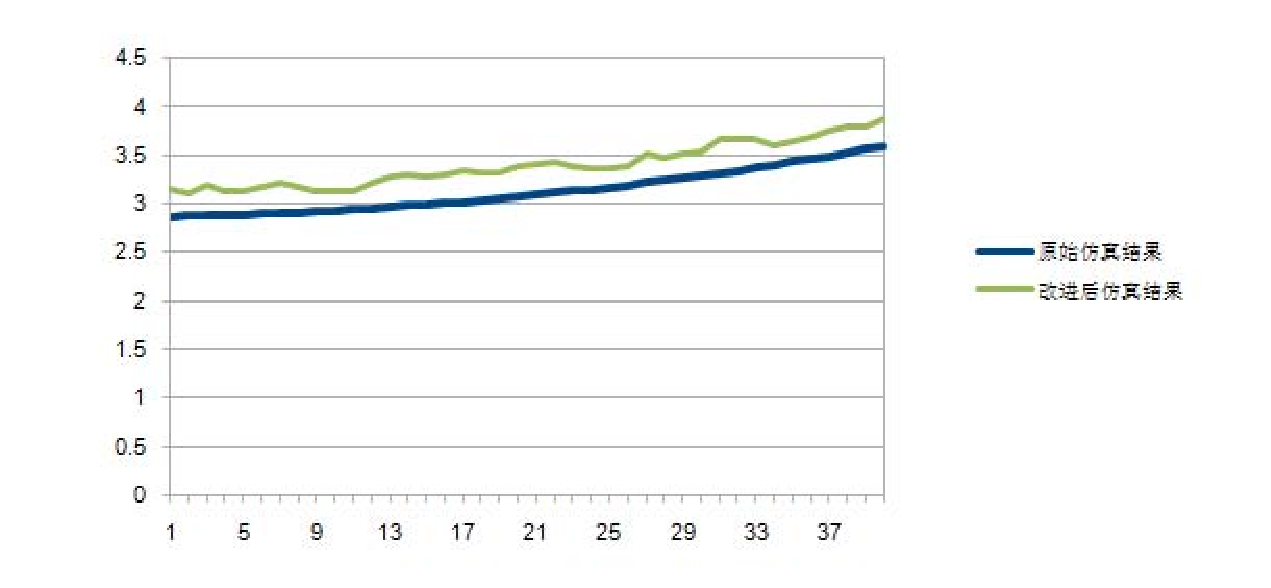
\includegraphics{improve5.pdf}}
  \caption{\small{\textbf{提升内容贡献者个体动机的仿真结果}}}
  \label{fig:improve5}
\end{figure}

图\ref{fig:improve6}是将所有的群体层次动机的初始值提升了$10\%$后的仿真结果。动机提升后个
体的贡献度同样有了一定的提高,同时随时间加速上升的趋势也要比提升前明显。
两个仿真的结果还表明,提升个体动机和人际间动机效果是一样
的。内容贡献者既重视在知识协同中获得心理上的满足感,同时也从与他人的互
动过程中获得良好的体验。

\begin{figure}[!htb]
  \centering
  \scalebox{0.65}{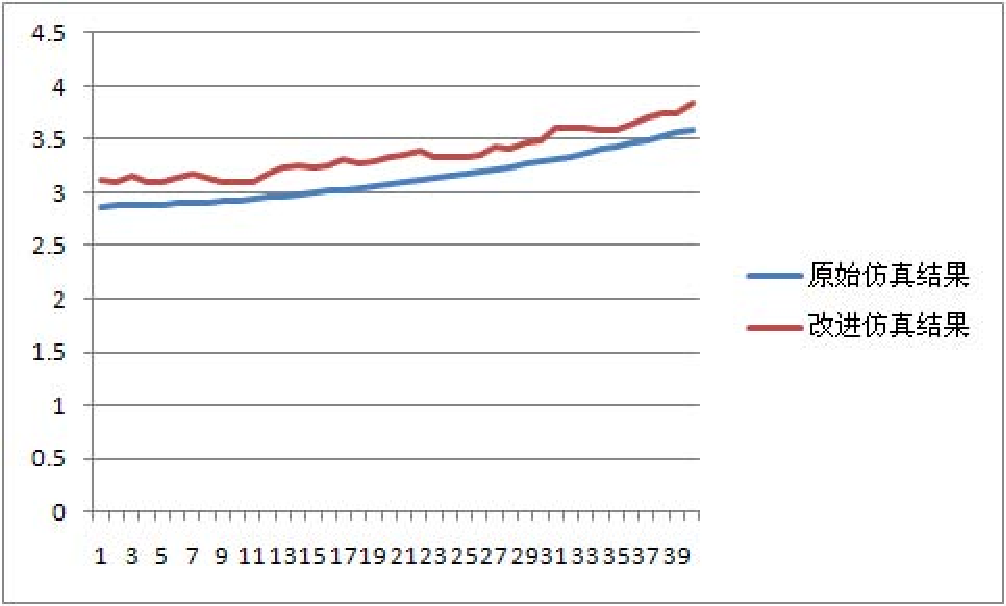
\includegraphics{improve6.pdf}}
  \caption{\small{\textbf{提升内容贡献者人际间动机的仿真结果}}}
  \label{fig:improve6}
\end{figure}

社区对于内容贡献者的激励可以从两方面展开。一方面,社区应该积极鼓励内容
协同者,重视他们的工作并及时给予积极的反馈,促进内容协同者动机水平的迅
速提升。另一方面,这类用户具有对社区的从属和依赖感,因此社区应采取措施
保护用户对社区的感情。尤其是当社区的规模不断扩大时,其他用户各种不合意的行为会
不断涌现出来,而内容贡献者对他人的行为要比领导者敏感的多。不断指定各种
制度、规定保障知识协同的顺利开展,已有的成果不被破坏,是保证内容贡献者
的知识协同动机不断提升的保证。

\subsection{内容维护者}
内容维护者在社区中属于积极参与,但是贡献水平较低,工作质量较差的群体。
其编辑的内容受到认可的程度要远远低于前三类用户。根据统计结果,内容维护
者的总贡献只相当于其正贡献值的$60\%$,这意味着有$40\%$的贡献未受到其他
协同者的承认。随着时间推移,负面效应
累计的影响越来于多,使得其月人均贡献度不断下降。仿真的结果显示贡献度呈
对数下降趋势,证明负反馈对其协同水平其主要作用。

负反馈之所以能够占据主导地位,是因为内容维护者对于负反馈的敏感程度要大
于正反馈的敏感程度。考虑到内容维护者的贡献还是以正贡献居多,如果个体更
看重正反馈的话是不可能使贡献度不断下降的。图是将所有的负反馈的转换系数
降低$35\%$后的仿真结果。降低转换系数意味着个体的负反馈的敏感程度下降,
由此可以检验其对个体动机的影响。仿真结果显示个体的贡献度变化趋势发生了
明显变化,由下降趋势转为缓慢上升,意味着正反馈占据了主导力量。

图\ref{fig:improve7}和图\ref{fig:improve8}进一步比较了个体动机因素和人际间动机因素对内容维护者的影响。
仿真分别降低个体层次动机的负反馈的转换系数和群体层次的动机负反馈的转换
系数各$10\%$。结果显示两种方案都使负反馈的力量减小,但是人际间动机改
变的程度较大,意味着提升内容维护者的贡献度的措施针对其群体层次的动机开展会更有效。

\begin{figure}[!htb]
  \centering
  \scalebox{0.65}{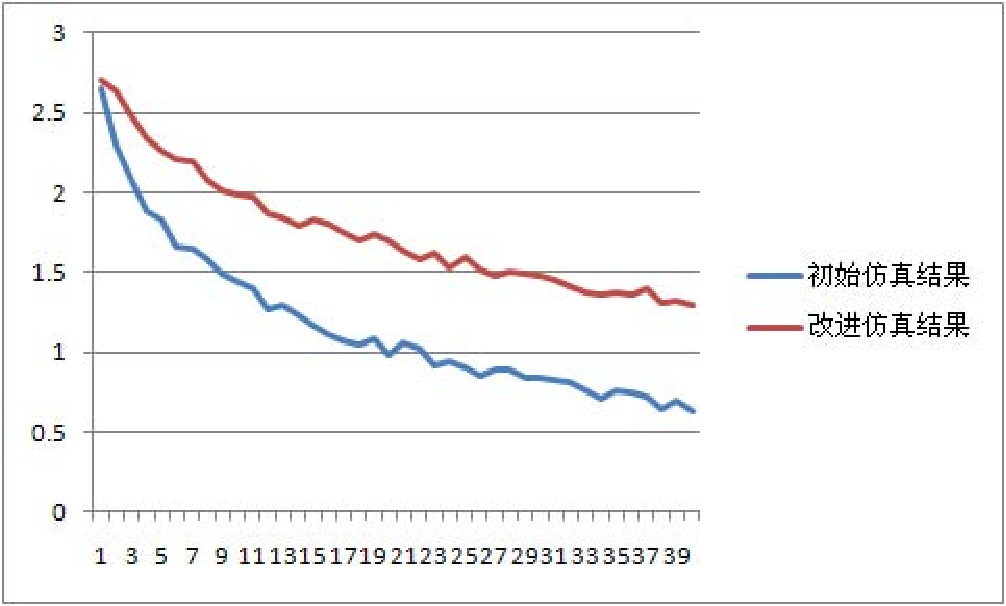
\includegraphics{improve7.pdf}}
  \caption{\small{\textbf{提升内容维护者个体动机的仿真结果}}}
  \label{fig:improve7}
\end{figure}

\begin{figure}[!htb]
  \centering
  \scalebox{0.65}{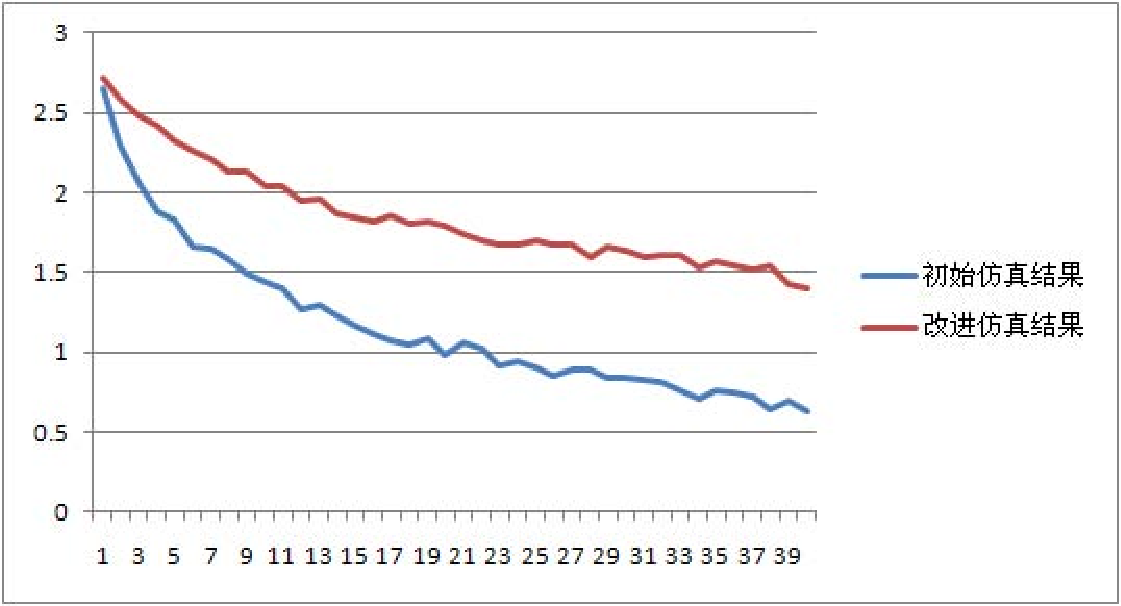
\includegraphics{improve8.pdf}}
  \caption{\small{\textbf{提升内容维护者个体动机的仿真结果}}}
  \label{fig:improve8}
\end{figure}
满足自身的社会需求是内容维护者参与社区的主要因素。内容维护者希望借由参
与社区感受到社区的温暖和支持,渴望获得社区的接纳和认同。同时,内容维护者自身的动机
水平偏低,害怕失败,尤其对于他人的行为比较敏感,动机水平容易受到外界因
素影响。这些特点决定了社区对其支持的方向应该是从保护其协同动
机入手,努力降低其对失败的关注程度,增加个体之间的协调和互动。社区管理
者应该鼓励用户之间多沟通,
多讨论,尤其是当拒绝某个人编辑的内容时应该尽力使其了解拒绝的理由、指明
改进的方向,帮助其提升编辑的水平。这样,参与者既感受到了来自于社区的支
持,同时可以将负面的感觉降低,转而多关注自身的成功,不断提升参与的信
心,使正反馈成为主导力
量。

\subsection{边缘用户}
边缘用户同内容维护者有着类似的行为模式,但是内容贡献度更低,参与次数更
少。边缘用户的月人均贡献是所有用户中唯一低于0的群体,并且变化趋势是加
速下降。边缘用户的正贡献和负贡献的比例基本是1:1,也就是说边缘用户的所
有用户贡献正负各一半,是所有用户中比例最接近的,负反馈对其的影响也是最
大的。

根据边缘用户的动机因素模型中存在着明显的负反馈环:当各体的动机降低是,
协同行为水平也会相应降低,这会导致负反馈的减少;负反馈的减少会增强个体
的动机。但是,边缘用户的行为特点显示负反馈环并未起到主导作用,这是由于
边缘用户参与的次数非常少,以至于他们不可能通过减少参与水平来达到提升个
体动机的目的。如果提升个体的动机,那么边缘用户将能够显著提升参与程度,
并转化为内容维护者,摆脱之前越不参与动机越低,动机越低越不
参与的恶性循环。

图\ref{fig:improve9}是将边缘用户的所有动机初始水平提升$30\%$所做的仿真实验。在提升初始动
机水平后,边缘用户的参与水平得到提高,并且在更多的参与中吸取了经验,熟
悉了编辑的规则和流程,提升了编辑的质量。这时边缘用户已经转化为内容贡献
者,内容贡献度的变化趋势也由加速下降转变为减速下降。仿真结果表明初始动
机水平较低是边缘用户最大的弱点,改善这一点将有助于其从社区的外围真正融
入到社区中。

\begin{figure}[!htb]
  \centering
  \scalebox{0.65}{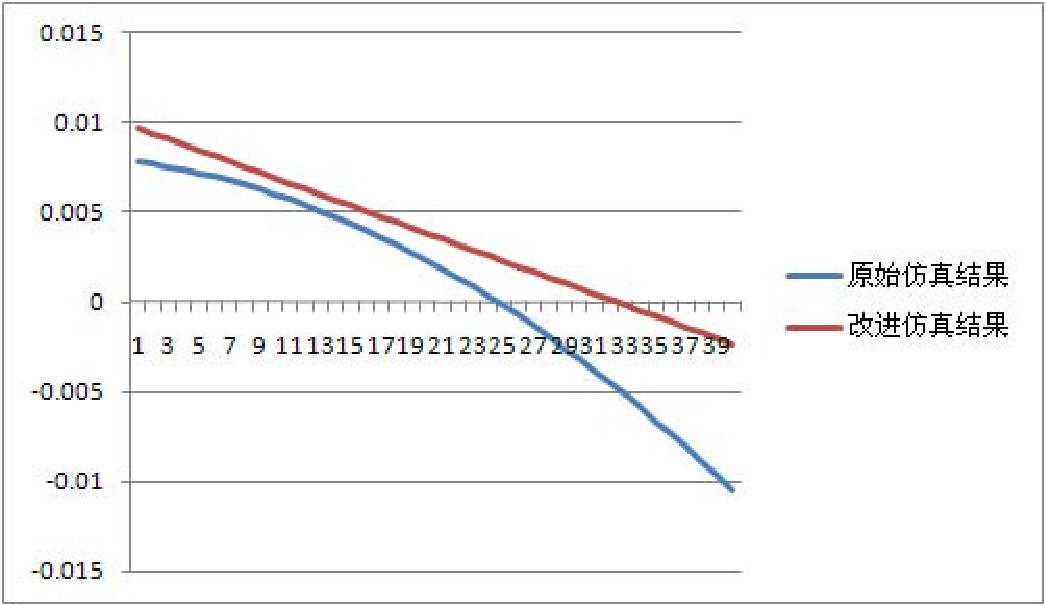
\includegraphics{improve9.pdf}}
  \caption{\small{\textbf{提升边缘用户动机的仿真结果}}}
  \label{fig:improve9}
\end{figure}

边缘用户是整个社区中参与动机最弱,参与程度最低的群体。运用各种手段提升
其参与动机,使其转变为其它类型的用户是社区的重要任务之一。社区可以采取
的措施包括鼓励用户多参与协同活动,可以设置一些实验性作品供用户练习、熟
悉,同时还不必考虑是否会得到负面反馈。准备各种示范材料、帮助手册用以提
升用户的编辑水平,帮助他们尽快适应协同编辑的模式。在宽松的环境下,边缘
用户容易培养自信,提升参与动机,同时提升编辑的质量。尽管绝大部分边缘用户在
其整个社区生涯中都不会改变其行为特点,但是社区仍然应该注重对边缘用户的关注。
社区只有拥有数量庞大的边缘用户才能不断涌现出高质量的用户。

\section{本章小结}

动机因素模型的建立为分析维基百科社区中的用户动机提供了有力的工具。仿真
的结果表明,动机模型能够较好地反应用户参与知识协同的动机。利用
系统动力学模型,不但揭示了不同动机因素对于用户行为的影响,还反映了行为
结果对于动机水平的影响,使得动机与行为间的关系形成了完整的闭环。在此基础上,进
一步针对不同类型用户的特点提出管理建议,并利用仿真模型验证改进的有效性。
社区建设者可以根据这些结果有针对性地做出改进,从而促进社区更好地发展。



%%% Local Variables: 
%%% mode: latex
%%% TeX-master: t
%%% End: 
